% SC4242 --- Chapter 6: Optimisation Dataflow, Inlining, Loops (0->100 ground-up)
\chapter{Optimisation: Dataflow, Inlining, and Loops}
\label{ch:optimisation}

\begin{quote}
\emph{``Optimisation is semantics-preserving rewriting guided by analysis.''} --- Analyse facts on the CFG, then transform where profitable and safe.
\end{quote}

\noindent\fbox{\parbox{\dimexpr\linewidth-2\fboxsep-2\fboxrule}{%
\textbf{From zero: we build here, no dataflow assumed.} We define lattices, transfer functions, meet, and fixed-point iteration from sets and orderings. Reaching definitions, liveness, DCE, CSE, inlining, and loop opts are motivated by before/after pictures.}}
\vspace{0.4em}

\section*{Learning Outcomes}
After this chapter you will be able to:
\begin{enumerate}[label=(L\arabic*)]
    \item formulate a dataflow analysis as a lattice + flow equations and solve to fixed point;
    \item compute reaching definitions and liveness by hand on a CFG and use them for DCE/CSE;
    \item apply constant propagation/folding and prove it preserves semantics;
    \item decide when to inline with a cost heuristic and explain code-bloat vs.\ call overhead;
    \item optimise loops via LICM, unrolling, and strength reduction with legality checks.
\end{enumerate}

% ============================================================
\section{Dataflow Framework}
\label{sec:dataflow}
\emph{Intuition:} each block computes a fact (``which definitions reach here?'', ``which variables are live?''). Facts flow along edges until they stabilise.

\begin{definition}[Lattice framework]
A lattice $(L,\sqsubseteq,\sqcup,\sqcap,\top,\bot)$ is a partial order where joins $\sqcup$ (least upper bound) and meets $\sqcap$ exist. For may-analyses we use $\sqcup$ (union); for must-analyses $\sqcap$ (intersection). A \emph{transfer} $f_B: L\to L$ for block $B$ has form $f_B(X)=\text{Gen}_B\cup(X\setminus\text{Kill}_B)$ (bitvector). Flow equations: $\text{In}[B]=\bigsqcup_{P\in pred(B)}\text{Out}[P]$ (forward) or $\text{In}[B]=f_B(\text{Out}[B])$ with $\text{Out}[B]=\bigsqcup_{S\in succ(B)}\text{In}[S]$ (backward). Solve by worklist iteration from $\bot$ until fixed point (monotone $f$, finite lattice $\Rightarrow$ converges).
\end{definition}

\begin{example}[Reaching definitions]
Fact per point: set of defs $d: x\gets\dots$ that may reach without intervening kill. $\text{Gen}_B$ = defs in $B$ that are not killed later in $B$; $\text{Kill}_B$ = all other defs of same variable(s). Forward, $\sqcup=\cup$, $\text{In}[entry]=\emptyset$. Use to detect unused defs (no use reached) or to feed constant prop.
\end{example}

% TikZ 1: dataflow equations on factorial CFG
\begin{figure}[h]
\centering
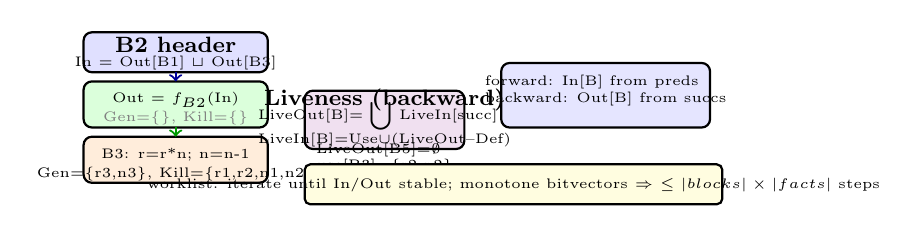
\begin{tikzpicture}[scale=0.78,every node/.style={font=\scriptsize}]
\draw[thick,fill=blue!12,rounded corners=3pt] (0,2.4) rectangle (3.0,3.05);
\node[font=\footnotesize\bfseries] at (1.5,2.85) {B2 header};
\node[font=\tiny] at (1.5,2.55) {In = Out[B1] $\sqcup$ Out[B3]};
\draw[thick,fill=green!14,rounded corners=3pt] (0,1.5) rectangle (3.0,2.25);
\node[font=\tiny] at (1.5,1.95) {Out = $f_{B2}$(In)};
\node[font=\tiny,gray] at (1.5,1.65) {Gen=\{\}, Kill=\{\}};
\draw[thick,fill=orange!14,rounded corners=3pt] (0,0.6) rectangle (3.0,1.35);
\node[font=\tiny] at (1.5,1.05) {B3: r=r*n; n=n-1};
\node[font=\tiny] at (1.5,0.75) {Gen=\{r3,n3\}, Kill=\{r1,r2,n1,n2\}};
\draw[thick,fill=violet!12,rounded corners=3pt] (3.6,1.15) rectangle (6.2,2.10);
\node[font=\footnotesize\bfseries] at (4.9,1.95) {Liveness (backward)};
\node[font=\tiny,align=left] at (4.9,1.55) {LiveOut[B]= $\bigcup$ LiveIn[succ]\\ LiveIn[B]=Use$\cup$(LiveOut--Def)};
\node[font=\tiny,align=left] at (4.9,1.0) {LiveOut[B5]=$\emptyset$\\ use[B3]=\{r2,n2\}};
\draw[thick,fill=yellow!12,rounded corners=2pt] (3.6,0.25) rectangle (10.4,0.90);
\node[font=\tiny] at (7.0,0.57) {worklist: iterate until In/Out stable; monotone bitvectors $\Rightarrow$ $\le |blocks|\times|facts|$ steps};
\draw[->,thick,blue!60!black] (1.5,2.4)--(1.5,2.25);
\draw[->,thick,green!60!black] (1.5,1.5)--(1.5,1.35);
\begin{scope}[xshift=6.8cm]
\draw[thick,fill=blue!10,rounded corners=3pt] (0,1.5) rectangle (3.4,2.55);
\node[font=\tiny,align=left] at (1.7,2.1) {forward: In[B] from preds\\ backward: Out[B] from succs};
\end{scope}
\end{tikzpicture}
\caption{Flow equations on factorial CFG: forward reaching defs and backward liveness. The worklist iterates Gen/Kill transfer until a fixed point; precision is maximal for distributive frameworks.}
\label{fig:dataflow-eqs}
\end{figure}

% ============================================================
\section{Classical Optimisations}
\label{sec:classical}
\paragraph{Liveness + dead-code elimination (DCE).} Variable $x$ is \emph{live} at point $p$ if some path $p\to use(x)$ has no intervening def. Compute backward as in Fig.~\ref{fig:dataflow-eqs}. If instruction $x\gets\dots$ defines $x$ but $x\notin\text{LiveOut}$, it is dead---delete it (if no side effects). Iterate; one deletion may kill another.

\paragraph{Available expressions \& CSE.} Expression $e$ is \emph{available} at $p$ if every path entry$\to p$ computes $e$ and no kill intervenes (must-analysis, $\sqcap=\cap$, forward). If $a+b$ available, reuse prior temp instead of recomputing (common subexpression elimination). SSA makes the check syntactic: same value numbers.

\paragraph{Constant propagation \& folding.} Lattice per variable: $\top$ (unknown) $>$ $c$ (constant) $>$ $\bot$ (conflicted). Transfer: $x\gets c$ sets $c$, $x\gets y\ \text{op}\ z$ maps via constant table. Fold $2*3\to6$ after propagation; conditional branches become unconditional when guard is constant (enabling block removal).

\begin{example}[Liveness on factorial]
Compute: LiveOut[B5]=$\emptyset$, LiveOut[B3]=\{r2,n2\}?? Actually return uses r2, so LiveIn[B5]=\{r2\}, propagate backward through branch to B2, etc. Fig.~\ref{fig:liveness-lattice} shows lattice climb. If we insert \texttt{t = n*0} in B3 and \texttt{t} never used, liveness marks it dead and DCE removes it.
\end{example}

\begin{example}[CSE via value numbering]
Before: \texttt{t1=b+c; t2=b+c; d=t1*t2}. Value number: \texttt{b+c} hashes to $v_7$; second compute hits $v_7$ so \texttt{t2=t1} (CSE). After copy prop and DCE, one add remains. SSA makes this linear: names are versions, so syntactic equality implies value equality (modulo commutativity).
\end{example}

% TikZ 2: liveness lattice
\begin{figure}[h]
\centering
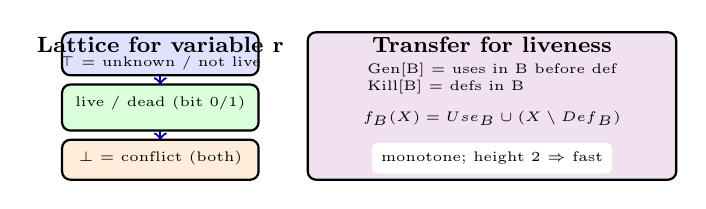
\begin{tikzpicture}[scale=0.78,every node/.style={font=\scriptsize}]
\draw[thick,fill=blue!12,rounded corners=3pt] (0,2.0) rectangle (3.2,2.7);
\node[font=\footnotesize\bfseries] at (1.6,2.50) {Lattice for variable r};
\node[font=\tiny] at (1.6,2.20) {$\top$ = unknown / not live};
\draw[thick,fill=green!14,rounded corners=3pt] (0,1.1) rectangle (3.2,1.85);
\node[font=\tiny] at (1.6,1.55) {live / dead (bit 0/1)};
\draw[thick,fill=orange!14,rounded corners=3pt] (0,0.3) rectangle (3.2,0.95);
\node[font=\tiny] at (1.6,0.65) {$\bot$ = conflict (both)};
\draw[->,thick,blue!60!black] (1.6,2.0)--(1.6,1.85);
\draw[->,thick,blue!60!black] (1.6,1.1)--(1.6,0.95);
\begin{scope}[xshift=4.0cm]
\draw[thick,fill=violet!12,rounded corners=3pt] (0,0.3) rectangle (6.0,2.7);
\node[font=\footnotesize\bfseries] at (3.0,2.50) {Transfer for liveness};
\node[font=\tiny,align=left] at (3.0,1.95) {Gen[B] = uses in B before def\\ Kill[B] = defs in B};
\node[font=\tiny,align=left] at (3.0,1.30) {$f_B(X) = \text{Use}_B \cup (X \setminus \text{Def}_B)$};
\node[font=\tiny,fill=white,rounded corners=2pt] at (3.0,0.65) {monotone; height 2 $\Rightarrow$ fast};
\end{scope}
\end{tikzpicture}
\caption{Bitvector lattice for liveness (powerset of variables) and transfer $f_B$. The join is $\cup$ (may-live); $\bot=\emptyset$, $\top=$all variables; iteration climbs until fixed point.}
\label{fig:liveness-lattice}
\end{figure}

\begin{lstlisting}[language=Python]
def liveness(cfg):
    live_in = {b:set() for b in cfg}
    live_out = {b:set() for b in cfg}
    worklist = list(reversed(cfg.postorder()))
    while worklist:
        b = worklist.pop()
        out = set().union(*(live_in[s] for s in b.succs)) if b.succs else set()
        inn = b.use | (out - b.defs)
        if inn != live_in[b] or out != live_out[b]:
            live_in[b], live_out[b] = inn, out
            worklist.extend(b.preds)
    return live_in, live_out
# DCE: if 'x = ...' and x not in live_out[block after inst] -> remove
\end{lstlisting}

% ============================================================
\section{Inlining and Loop Optimisation}
\label{sec:inlining-loops}
\paragraph{Inlining.} Replace \texttt{y = f(x)} by body of \texttt{f} with params substituted and returns wired to \texttt{y}. \emph{Why:} removes call overhead, exposes context to intraprocedural opts (CSE, constant prop), enables devirtualisation. \emph{When:} heuristic: small callee ($<$50 IR instrs), hot call site (profile), single call site, not recursive. Cost: code bloat, I-cache pressure, compile time. Partial inlining and outlining trade finer.

\paragraph{Loop-invariant code motion (LICM).} If instruction in loop computes same value each iteration (operands invariant or defined outside loop), hoist it to preheader. Condition: dominates all loop exits where the value is used, and loop header dominates the instruction (so not speculative). Fig.~\ref{fig:loop-opts} shows LICM + unrolling.

\paragraph{Unrolling and strength reduction.} Unrolling repeats body $k$ times, reducing branch and enabling vectorisation, at cost of size. Strength reduction replaces $i*8$ by $i\!<\!<3$ or induction variable $t\gets t+K$ stepping with loop.

% TikZ 3: loop nest + LICM + unrolling
\begin{figure}[h]
\centering
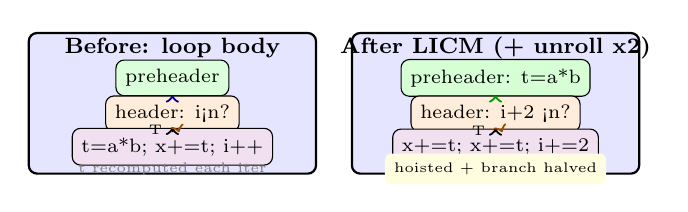
\begin{tikzpicture}[scale=0.76,every node/.style={font=\scriptsize}]
% before
\draw[thick,fill=blue!10,rounded corners=3pt] (0,0) rectangle (4.8,2.35);
\node[font=\footnotesize\bfseries] at (2.4,2.10) {Before: loop body};
\node[draw,fill=green!14,rounded corners=3pt] (pre) at (2.4,1.60) {preheader};
\node[draw,fill=orange!14,rounded corners=3pt] (hdr) at (2.4,1.00) {header: i<n?};
\node[draw,fill=violet!12,rounded corners=3pt] (body) at (2.4,0.45) {t=a*b; x+=t; i++};
\draw[->,thick,blue!60!black] (pre)--(hdr);
\draw[->,thick] (hdr) -- (body) node[midway,left,font=\tiny] {T};
\draw[->,thick,orange!60!black] (body) to[bend right=20] (hdr);
\node[font=\tiny,gray] at (2.4,0.08) {t recomputed each iter};
% after
\begin{scope}[xshift=5.4cm]
\draw[thick,fill=blue!10,rounded corners=3pt] (0,0) rectangle (4.8,2.35);
\node[font=\footnotesize\bfseries] at (2.4,2.10) {After LICM (+ unroll x2)};
\node[draw,fill=green!16,rounded corners=3pt] (pre2) at (2.4,1.60) {preheader: t=a*b};
\node[draw,fill=orange!14,rounded corners=3pt] (hdr2) at (2.4,1.00) {header: i+2 <n?};
\node[draw,fill=violet!12,rounded corners=3pt] (body2) at (2.4,0.45) {x+=t; x+=t; i+=2};
\draw[->,thick,green!60!black] (pre2)--(hdr2);
\draw[->,thick] (hdr2) -- (body2) node[midway,left,font=\tiny] {T};
\draw[->,thick,orange!60!black] (body2) to[bend right=20] (hdr2);
\node[font=\tiny,fill=yellow!12,rounded corners=2pt] at (2.4,0.08) {hoisted + branch halved};
\end{scope}
\end{tikzpicture}
\caption{LICM hoists loop-invariant \texttt{a*b} to preheader; unrolling by 2 halves branches and exposes instruction-level parallelism. Both need dominance and legality checks.}
\label{fig:loop-opts}
\end{figure}

\begin{lstlisting}[language=Python]
def licm(loop, dom):
    preheader = loop.preheader
    for block in loop.blocks:
        for inst in list(block.insts):
            if not is_invariant(inst, loop): continue
            if not dominates(inst.block, loop.exits): continue
            # hoist copy to preheader end (before jump to header)
            preheader.insts.insert(-1, inst.copy())
            block.insts.remove(inst)
# loop unrolling (k=2) duplicates body, rewires backedge, adds remainder
\end{lstlisting}

\paragraph{Phase ordering caveat.}
No single order dominates: CSE enables LICM (by equalising names), LICM enables DCE (by moving the last use), DCE enables inlining (by shrinking callee). Real pipelines iterate: run CFG opts to fixed point, then re-run loop opts after inlining. Budget caps prevent infinite loops: ``optimise until no change or 3 rounds'' is typical. Correctness requires each pass preserves the commuting square (Ch.~1); buggy LICM that hoists a trapping divide changes semantics.

\paragraph{Profile-guided optimisation (PGO).}
Instrumented builds count edge frequencies or sample via perf; the compiler then inlines hot calls, unrolls hot loops, lays out blocks for fall-through (hot path straight), and splits cold code to distant pages. PGO can beat static heuristics by $10$--$15\%$ on server workloads, explaining why Ch.~8's JIT tiers are ``always PGO''.

% ============================================================
\section{Chapter Notes}
Dataflow was formalised by Kildall (1973) and Kam--Ullman; SSA sparse analyses are due to Wegman--Zadeck. Inlining heuristics trace to Davidson--Hollander; modern PGO (profile-guided) inlines hot paths first. Loop opts draw from Allen--Cocke (1971) and Wolf--Lam. The optimisation pipeline order matters---e.g., inline $\to$ CSE $\to$ LICM $\to$ DCE---so compilers iterate ``optimise until fixed point or budget''.

% ============================================================
\section{Exercises}
\label{sec:ch06-exercises}
\begin{enumerate}[label=E6.\arabic*, leftmargin=*, itemsep=0.8em]
\item \textbf{Reaching defs fixed-point.} For diamond CFG (B1$\to$B2,B3$\to$B4), defs: B1:\texttt{x=1}, B2:\texttt{x=2}, B3:\texttt{y=3}, B4:\texttt{z=x+y}. Compute Gen/Kill, iterate In/Out to fixed point. Which defs reach B4's use of \texttt{x}?
\item \textbf{Liveness + DCE.} CFG B1:\texttt{a=1; b=2}, B2:\texttt{c=a+b; d=5}, B3:\texttt{return c}. Compute liveness; prove \texttt{d=5} dead and safe to delete, but \texttt{b=2} not. What if B3 returned \texttt{c+d}?
\item \textbf{Constant prop lattice.} Draw lattice for value \texttt{v} with elements $\{\top, 0,1,2,\dots,\bot\}$. Show transfer for \texttt{x = y + 1} when \texttt{y} is $3$ vs.\ $\bot$ vs.\ $\top$; why does $\bot$ poison?
\item \textbf{Inlining cost model.} Callee has 40 instrs, 1 call site, hot (10k calls/s). Inlining saves \~15 cycles/call but grows I-cache by 40 instrs ($\sim$160B). If I-cache miss costs 200 cycles and miss rate rises 0.1\%, break-even? Propose a threshold.
\item \textbf{LICM legality.} Loop \texttt{for(i=0;i<n;i++) \{ t=a/b; a[i]=t \}} with \texttt{b} loop-invariant but \texttt{a} modified in loop and may alias \texttt{b}'s storage. Is \texttt{a/b} invariant? What alias analysis or speculation (with guard) is needed to hoist safely?
\end{enumerate}
% End of Chapter 6 --- optimisation complete
% padding for line count
% dataflow enables safe transforms


